\documentclass[12pt]{article}
\usepackage[margin = 2cm]{geometry}

\usepackage{linguex}
\usepackage[svgnames]{xcolor}
\usepackage{tikz, pgfplots}
\usetikzlibrary{backgrounds,fit}
\usetikzlibrary{calc}

% \usepackage[backend=biber,
%         bibstyle=biblatex-sp-unified,
%         citestyle=sp-authoryear-comp,
%         maxcitenames=3,
%         maxbibnames=99]{biblatex}

\usepackage[natbib=true,
            style=authoryear-comp,
            backend=bibtex,
            doi=false,
            url=false,
            sortcites=false,
            maxcitenames=3, 
            maxbibnames=99]{biblatex}

\addbibresource{bibliography.bib}

%\usepackage[T1]{fontenc}

\usepackage{textcomp}
\usepackage{mathptmx}
\usepackage{booktabs,multirow}
\usepackage{todonotes}
\usepackage{nicefrac}
\usepackage{amsmath}
\usepackage{amssymb,amsmath}
\usepackage{subcaption}
\usepackage{wrapfig} 
\usepackage{float} 
\usepackage{xspace}


%%%% some commands

\newcommand{\den}[1]{\left [\! \left [ #1 \right ]\! \right]}
\newcommand{\set}[1]{\left\{#1\right\}}
\newcommand{\tuple}[1]{\left \langle #1\right\rangle}
\newcommand{\card}[1]{\left \lvert \, #1 \, \right\rvert}
\newcommand{\abs}[1]{\lvert #1 \rvert}
\newcommand{\setbar}{\ensuremath{\thinspace \mid \thinspace}}
\newcommand{\probbar}{\ensuremath{\mid}}
\DeclareMathOperator{\expo}{exp}
\newcommand{\acro}[1]{\textsc{#1}\xspace}
\newcommand{\rel}{\acro{Rel}}
\newcommand{\com}{\acro{Com}}
\newcommand{\pri}{\acro{Pri}}
\newcommand{\exh}{\acro{Exh}}
\newcommand{\xor}{\acro{XOr}}

\newcommand{\mygray}[1]{\textcolor{gray}{#1}}
\definecolor{Red}{RGB}{178,34,34}
\newcommand{\mf}[1]{\textcolor{Red}{[#1]}} 



\begin{document}

\pagestyle{empty}

\noindent \large\textbf{Exclusive disjunction: implicature or \dots} \\[3pt]\normalsize
Michael Franke (Universit\"{a}t T\"{u}bingen) \\[0pt] Bob van Tiel (Universit\'{e} Libre de Bruxelles) \\

\medskip

\noindent \textbf{Introduction.} Exclusive readings of disjunctions are frequently treated as a scalar implicature
arising from the competition of lexical alternatives \emph{or} and \emph{and}, parallel to the
case of \emph{some} and \emph{all}. However, there is recent experimental evidence for the
assumption that the strength of scalar inferences can vary substantially between different
scalar items \citep[e.g.][]{Tielvan-TielMiltenburgvan-Miltenburg2014:Scalar-Diversit} and be
affected by multiple contextual factors in subtle ways
\citep[e.g.][]{Degen2015:Investigating-t}. The main question that we would like to address
experimentally in this paper is therefore: is the strength of exclusive readings of
disjunctions influenced by contextual factors in the way that a scalar implicature account
would predict?

Many factors may have an effect on the strength of scalar inferences. We will focus here on
three factors, for reasons of theoretical interest: (i) whether the scalar inference is
\emph{relevant} information for the listener (factor \rel); whether the speaker is
\emph{competent}, i.e., she knows whether a stronger alternative statement would be true
(factor \com), and (iii), although this is usually not discussed prominently in the theoretical
literature, whether common sense expectations make the propositional content of a scalar
inference \emph{a priori likely} (factor \pri).

Different theoretical accounts of scalar implicatures may assign different weights to these
factors, but, arguably, most would acknowledge that these factors play a role. For instance,
standard Gricean(-like) reasoning could make relevance of information and the speaker's
competence necessary conditions for the derivation of a scalar implicature, but also see a role
for prior expectations. A game-theoretic or probabilistic approach might put particular
emphasis on the role of prior expectations instead. In grammatical approaches potential scalar
implicatures are generated as parses of sentences and some disambiguation procedure selects
(contextually) preferred parses. Here, the relevance of alternatives is often flagged as
important, but it is not strange to think that the disambiguation procedure is sensitive to the
other factors as well: for instance, it may weigh in the contextual plausibility of ignorance
inferences that different parses would give rise to \citep[e.g.][]{Fox2007:Free-Choice-and}.

Across many prominent theoretical frameworks, we would therefore expect that strength of scalar
inferences should be higher (i) the more contextual relevance is attributed to the stronger
alternative, (ii) the more likely the speaker is taken to know whether the stronger alternative
is true, and (iii) the less likely it is \emph{a priori} that the stronger alternative is
true. If this pattern is empirically confirmed for some scalar inferences, but not for others
that would be surprising, and potential evidence against a homogeneous theoretical treatment.

% \begin{enumerate}
% \item the higher the contextual relevance of the information conveyed by the scalar alternative
%   is to the listener, the more salient the scalar inference should be;
% \item the more likely the speaker is thought to know whether the scalar alternative is true,
%   the more strongly the scalar inference should suggest itself;
% \item the less likely the scalar alternative is true, the stronger the scalar implicature
%   should be.
% \end{enumerate}

\medskip

\noindent \textbf{Experiment~1.}\ We tested the effects of factors \rel, \com and \pri on the
robustness of exclusive readings. Materials consisted of 16 vignettes involving two characters
$S$ and $H$. Each vignette introduced some background scenario and, except for \pri-conditions
(see below), ended with $S$ uttering a sentence of the form ``$A$ or $B$.'' We classified each
vignette based our own intuition as either high or low in each of \rel, \com and \pri, and
created 2 vignettes for all 8 theoretically possible vignette types, i.e., intuitively high/low
factor combinations. Since our own intuitive classification might not accord with the
perception of our experimental subjects, we obtained empirical measures for \rel, \com and \pri
and used these as explanatory factors for the measured strength of exclusive readings
(\xor). To do so, each vignette was associated with five statements: three control statements
and four types of target statements, which aimed at \rel (``It is important for $H$ to know
whether $A$ and $B$''), \com (``$S$ knows whether $A$ and $B$''), \pri (``If $A$, it is likely
that $B$ as well'' and ``If $B$, it is likely that $A$ as well''),\footnote{Statements for \pri
  were formulated as pairs of conditionals, rather than as single statements about the
  conjunction ``$A$ and $B$,'' because the latter may be very unlikely in a context where also
  many other options $C$, $D$, \dots are conceivable.  As a result, we might not obtain
  judgements of \emph{a priori} plausibility that compare reliably across vignettes: a low
  rating for ``$A$ and $B$'' could be the result of comparing it to $C$, $D$, etc., in one
  case, and of considering it unlikely that both $A$ and $B$ hold if at least one of them does
  in another context. To avoid this issue, we used pairs of conditionals.} and \xor (``From
what $S$ said we may conclude that not both $A$ and $B$'').

200 participants, recruited via MTurk, each read 8 random vignettes, one of each vignette
type. Each vignette was followed by two statements: first a control statement, then one target
statement out of \rel, \com, \pri or \xor. (Trials probing for \pri were special: they did not
show $S$'s utterance of a disjunction and presented both of its target sentences in random
sequence.) Participants indicated how likely the statement was by adjusting a continuous slider
bar whose endpoints were labeled ``Certainly false'' to ``Certainly true.'' Responses to
controls clearly showed that participants paid attention to the vignettes and understood the
task (same for follow-up experiments). Slider ratings were coded as reals in
$[0;1]$. Figure~\ref{fig:correlationsExp1} plots per-vignette means of \xor-ratings against
those of \rel, \com and \pri. Our main results are foreshadowed by visual inspection: \rel does
not seem to be a good predictor of \xor; \com and \pri do, but the correlation between \com and
\xor is not as expected.

\begin{figure}[tb]
  \centering

  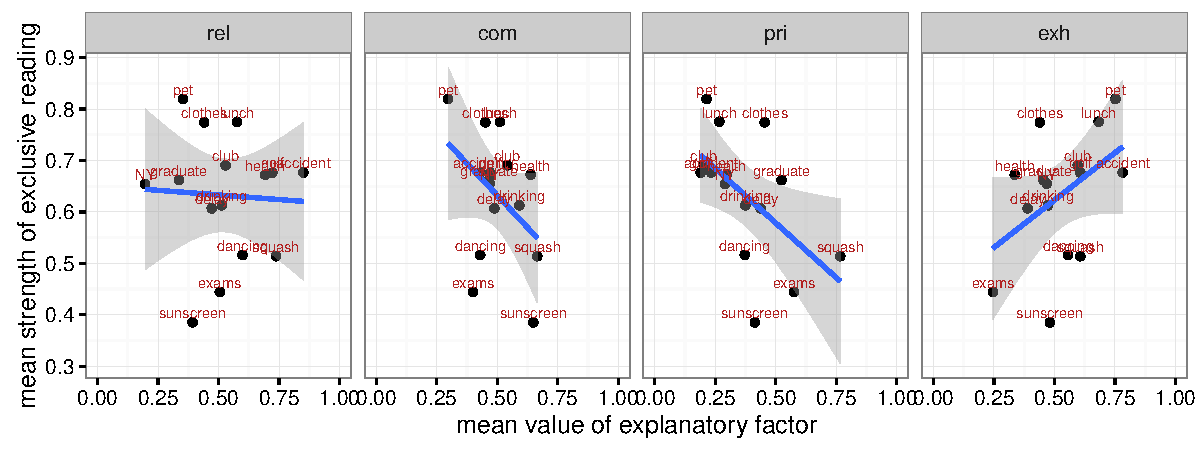
\includegraphics[width = 0.75\textwidth]{../01_paper_draft/pics/correlationExp1and3.pdf}
  
  \caption{Per-vignette means of implicature rating vs. per-vignette means of factor ratings in
    Exp.~1 \& 3}
  \label{fig:correlationsExp1}
\end{figure}

To test factor influence, we looked at linear regression models predicting \xor ratings from
by-vignette means of ratings for \rel, \com and \pri as main factors. Bayes factor model
comparison \citep[e.g.][]{KassRaftery1995:Bayes-Factors}, which weighs in likelihood and model
complexity, clearly identified two equally favored models that were significantly better than
all competitors:\footnote{Non-Bayesian analyses and more complex models involving interactions
  and by-participant intercepts support our main conclusions, so that we report only the
  simplest analyses here (similarly for follow up experiments).} one containing only \pri and
one containing \pri and \com. Estimates of coefficients indicated that both \pri and \com had
significant effects, but, critically, the effect of \com went in the opposite direction to what
an implicature-based approach predicts: the perceived strength of the exclusive reading
\emph{decreased} with the perceived competence of the speaker.% In effect, our
% analysis and data suggest that the prior probability of the \emph{and}-alternative is the
% decisive predictor of exclusive-\emph{or} strength, and, although it does have a slight
% explanatory effect, competence of the speaker influenced strength of exclusive-\emph{or} in the
% wrong direction.

How to explain the surprising negative effect of competence? Perhaps the most parsimonious
explanation would be to attribute it to methodological flaws. That is, perhaps our manipulation
did not measure what we assumed it measured. In order to address that possibility we replicated
Exp.~1 using vignettes with \emph{some}, which may license an upper-bounding inference to
the exclusion of \emph{all}. The status of this inference as a scalar implicature is less
controversial than in the case of exclusive-\emph{or}. Hence, \emph{some} provides a baseline
against which the results for \emph{or} can be contrasted.

\medskip

\noindent \textbf{Experiment~2.}\ Design and procedure of Exp.~2 was analogous to Exp.~1, but
used different vignettes with utterances containing \emph{some} instead of \emph{or}. Bayes
factor comparison of regression models showed that the optimal model for predicting the
strength of the upper-bounding inference contained both \pri and \com. Posterior estimates of
coefficients indicated, in this case, that the effect of \com went in the ``right'' direction:
the inference from \emph{some} to \emph{not all} was considered more robust if the speaker was
judged to be competent about the truth of the \emph{all}-alternative.

Taken together, the results of Exp.~1 and 2 indicate it might be a mistake to assume a
homogenous theoretical treatment of exclusive-\emph{or} and the upper-bounded inference
associated with \emph{some}. Assuming that the upper-bounded inference associated with
\emph{some} is a scalar implicature, one would then require an alternative treatment for
exclusive-\emph{or}. One such treatment is tentatively considered by
\citet{Fox2007:Free-Choice-and}. He suggests that exclusive-\emph{or} may come about by
exhaustifying the individual disjuncts rather than the disjunction as a whole. That is, ``$A$
or $B$'' might be interpreted as ``Only $A$ or only $B$,'' which excludes the possibility that
both $A$ and $B$ are true. If this account is correct, we might expect that the strength of
exclusive-\emph{or} is an increasing function of the strength of the exhaustive inference
associated with an utterance of the individual disjuncts, i.e. the inferences from ``$A$'' and
``$B$'' to ``only $A$'' and ``only $B$.'' This prediction was tested in Exp.~3.

\medskip

\noindent \textbf{Experiment~3.} Exp.~3 used the 16 vignettes from Exp.~1, changing only the
final utterance from a disjunction (``$A$ or $B$'') to an utterance of one of the disjuncts
(``$A$'' respectively ``$B$''). Each vignette was associated with four statements: three
control statements and one target statement probing for exhaustive interpretation of individual
disjuncts (``From what $S$ said we may conclude that $B$ is not true as well'' and ``From what
$S$ said we may conclude that $A$ is not true as well''). 130 participants each read 6
vignettes that were followed by one control and one target statement.

Mean ratings, per vignette, of target statements were added as an additional predictor \exh
(see Figure~\ref{fig:correlationsExp1}). Bayes factors in favor of the most preferred models
from Exp.~1 over a model that only contains \exh are about 5.24 and 5.63. This is just above
the threshold of 5 for Bayes factors to indicate substantial evidence in favor of a model, as
proposed by \citet{Jeffreys1961:Theory-of-Proba}. A model that uses both \pri and \exh as main
factors is just as credible, given the data, as a model with only \pri. Our data therefore
suggest that \pri might be the most reliable predictor of \xor, but \exh follows closely on its
heals. The inclusion of \exh does not lead us to revise our previous conclusions about \com and
\rel: the former is ``wrongly'' correlated with \xor; \rel is irrelevant.

\medskip

\noindent \textbf{Conclusion.}\ The behaviour of \emph{or} differs in some marked ways from the
behaviour of \emph{some} and more generally from what one would expect if exclusive-\emph{or}
were a scalar implicature. In particular, the strength of exclusive-\emph{or} did not increase
with the competence of the speaker about the \emph{and}-alternative; rather, the effect was the
other way around. This squares with the theoretically-motivated skepticism expressed by
\citet{Geurts2006:Exclusive-disju} about the status of exclusive-\emph{or} as scalar
implicature. On the positive side, our results indicate that strength of exclusive-\emph{or}
clearly seem to be influenced by prior expectations, and these also affect the strength of
\emph{some-but-not-all}-inferences. On the other hand, our results leave open the theoretically
interesting alternative that exclusive-\emph{or} might be the outcome of reading each disjunct
exhaustively. Finally, relevance failed to influence the strength of either exclusive-\emph{or}
or the upper-bounded inference associated with \emph{some}. This finding conflicts with the
received opinion about relevance, but is in line with recent experimental results suggesting a
marginal role for relevance in the derivation of scalar implicature
\citep[e.g.][]{Zondervan2010:Scalar-Implicat}.


% \newpage




% \printbibliography 


\end{document}
